\documentclass[]{book}
\usepackage{lmodern}
\usepackage{amssymb,amsmath}
\usepackage{ifxetex,ifluatex}
\usepackage{fixltx2e} % provides \textsubscript
\ifnum 0\ifxetex 1\fi\ifluatex 1\fi=0 % if pdftex
  \usepackage[T1]{fontenc}
  \usepackage[utf8]{inputenc}
\else % if luatex or xelatex
  \ifxetex
    \usepackage{mathspec}
  \else
    \usepackage{fontspec}
  \fi
  \defaultfontfeatures{Ligatures=TeX,Scale=MatchLowercase}
\fi
% use upquote if available, for straight quotes in verbatim environments
\IfFileExists{upquote.sty}{\usepackage{upquote}}{}
% use microtype if available
\IfFileExists{microtype.sty}{%
\usepackage{microtype}
\UseMicrotypeSet[protrusion]{basicmath} % disable protrusion for tt fonts
}{}
\usepackage[margin=1in]{geometry}
\usepackage{hyperref}
\hypersetup{unicode=true,
            pdftitle={Statistik},
            pdfauthor={Thomas Petersen},
            pdfborder={0 0 0},
            breaklinks=true}
\urlstyle{same}  % don't use monospace font for urls
\usepackage{natbib}
\bibliographystyle{apalike}
\usepackage{color}
\usepackage{fancyvrb}
\newcommand{\VerbBar}{|}
\newcommand{\VERB}{\Verb[commandchars=\\\{\}]}
\DefineVerbatimEnvironment{Highlighting}{Verbatim}{commandchars=\\\{\}}
% Add ',fontsize=\small' for more characters per line
\usepackage{framed}
\definecolor{shadecolor}{RGB}{248,248,248}
\newenvironment{Shaded}{\begin{snugshade}}{\end{snugshade}}
\newcommand{\AlertTok}[1]{\textcolor[rgb]{0.94,0.16,0.16}{#1}}
\newcommand{\AnnotationTok}[1]{\textcolor[rgb]{0.56,0.35,0.01}{\textbf{\textit{#1}}}}
\newcommand{\AttributeTok}[1]{\textcolor[rgb]{0.77,0.63,0.00}{#1}}
\newcommand{\BaseNTok}[1]{\textcolor[rgb]{0.00,0.00,0.81}{#1}}
\newcommand{\BuiltInTok}[1]{#1}
\newcommand{\CharTok}[1]{\textcolor[rgb]{0.31,0.60,0.02}{#1}}
\newcommand{\CommentTok}[1]{\textcolor[rgb]{0.56,0.35,0.01}{\textit{#1}}}
\newcommand{\CommentVarTok}[1]{\textcolor[rgb]{0.56,0.35,0.01}{\textbf{\textit{#1}}}}
\newcommand{\ConstantTok}[1]{\textcolor[rgb]{0.00,0.00,0.00}{#1}}
\newcommand{\ControlFlowTok}[1]{\textcolor[rgb]{0.13,0.29,0.53}{\textbf{#1}}}
\newcommand{\DataTypeTok}[1]{\textcolor[rgb]{0.13,0.29,0.53}{#1}}
\newcommand{\DecValTok}[1]{\textcolor[rgb]{0.00,0.00,0.81}{#1}}
\newcommand{\DocumentationTok}[1]{\textcolor[rgb]{0.56,0.35,0.01}{\textbf{\textit{#1}}}}
\newcommand{\ErrorTok}[1]{\textcolor[rgb]{0.64,0.00,0.00}{\textbf{#1}}}
\newcommand{\ExtensionTok}[1]{#1}
\newcommand{\FloatTok}[1]{\textcolor[rgb]{0.00,0.00,0.81}{#1}}
\newcommand{\FunctionTok}[1]{\textcolor[rgb]{0.00,0.00,0.00}{#1}}
\newcommand{\ImportTok}[1]{#1}
\newcommand{\InformationTok}[1]{\textcolor[rgb]{0.56,0.35,0.01}{\textbf{\textit{#1}}}}
\newcommand{\KeywordTok}[1]{\textcolor[rgb]{0.13,0.29,0.53}{\textbf{#1}}}
\newcommand{\NormalTok}[1]{#1}
\newcommand{\OperatorTok}[1]{\textcolor[rgb]{0.81,0.36,0.00}{\textbf{#1}}}
\newcommand{\OtherTok}[1]{\textcolor[rgb]{0.56,0.35,0.01}{#1}}
\newcommand{\PreprocessorTok}[1]{\textcolor[rgb]{0.56,0.35,0.01}{\textit{#1}}}
\newcommand{\RegionMarkerTok}[1]{#1}
\newcommand{\SpecialCharTok}[1]{\textcolor[rgb]{0.00,0.00,0.00}{#1}}
\newcommand{\SpecialStringTok}[1]{\textcolor[rgb]{0.31,0.60,0.02}{#1}}
\newcommand{\StringTok}[1]{\textcolor[rgb]{0.31,0.60,0.02}{#1}}
\newcommand{\VariableTok}[1]{\textcolor[rgb]{0.00,0.00,0.00}{#1}}
\newcommand{\VerbatimStringTok}[1]{\textcolor[rgb]{0.31,0.60,0.02}{#1}}
\newcommand{\WarningTok}[1]{\textcolor[rgb]{0.56,0.35,0.01}{\textbf{\textit{#1}}}}
\usepackage{longtable,booktabs}
\usepackage{graphicx,grffile}
\makeatletter
\def\maxwidth{\ifdim\Gin@nat@width>\linewidth\linewidth\else\Gin@nat@width\fi}
\def\maxheight{\ifdim\Gin@nat@height>\textheight\textheight\else\Gin@nat@height\fi}
\makeatother
% Scale images if necessary, so that they will not overflow the page
% margins by default, and it is still possible to overwrite the defaults
% using explicit options in \includegraphics[width, height, ...]{}
\setkeys{Gin}{width=\maxwidth,height=\maxheight,keepaspectratio}
\usepackage[normalem]{ulem}
% avoid problems with \sout in headers with hyperref:
\pdfstringdefDisableCommands{\renewcommand{\sout}{}}
\IfFileExists{parskip.sty}{%
\usepackage{parskip}
}{% else
\setlength{\parindent}{0pt}
\setlength{\parskip}{6pt plus 2pt minus 1pt}
}
\setlength{\emergencystretch}{3em}  % prevent overfull lines
\providecommand{\tightlist}{%
  \setlength{\itemsep}{0pt}\setlength{\parskip}{0pt}}
\setcounter{secnumdepth}{5}
% Redefines (sub)paragraphs to behave more like sections
\ifx\paragraph\undefined\else
\let\oldparagraph\paragraph
\renewcommand{\paragraph}[1]{\oldparagraph{#1}\mbox{}}
\fi
\ifx\subparagraph\undefined\else
\let\oldsubparagraph\subparagraph
\renewcommand{\subparagraph}[1]{\oldsubparagraph{#1}\mbox{}}
\fi

%%% Use protect on footnotes to avoid problems with footnotes in titles
\let\rmarkdownfootnote\footnote%
\def\footnote{\protect\rmarkdownfootnote}

%%% Change title format to be more compact
\usepackage{titling}

% Create subtitle command for use in maketitle
\newcommand{\subtitle}[1]{
  \posttitle{
    \begin{center}\large#1\end{center}
    }
}

\setlength{\droptitle}{-2em}

  \title{Statistik}
    \pretitle{\vspace{\droptitle}\centering\huge}
  \posttitle{\par}
    \author{Thomas Petersen}
    \preauthor{\centering\large\emph}
  \postauthor{\par}
      \predate{\centering\large\emph}
  \postdate{\par}
    \date{2018-07-11}

\usepackage{booktabs}
\usepackage{amsthm}
\makeatletter
\def\thm@space@setup{%
  \thm@preskip=8pt plus 2pt minus 4pt
  \thm@postskip=\thm@preskip
}
\makeatother

\usepackage{amsthm}
\newtheorem{theorem}{Theorem}[chapter]
\newtheorem{lemma}{Lemma}[chapter]
\theoremstyle{definition}
\newtheorem{definition}{Definition}[chapter]
\newtheorem{corollary}{Corollary}[chapter]
\newtheorem{proposition}{Proposition}[chapter]
\theoremstyle{definition}
\newtheorem{example}{Example}[chapter]
\theoremstyle{definition}
\newtheorem{exercise}{Exercise}[chapter]
\theoremstyle{remark}
\newtheorem*{remark}{Remark}
\newtheorem*{solution}{Solution}
\begin{document}
\maketitle

{
\setcounter{tocdepth}{1}
\tableofcontents
}
\hypertarget{forudstninger}{%
\chapter{Forudsætninger}\label{forudstninger}}

\hypertarget{Settings}{}

\hypertarget{TopBar}{}
\hypertarget{Sentry_label}{}
\protect\hypertarget{Sentry_label_span}{}{Member
Login}\protect\hypertarget{downArrow}{}{}

\hypertarget{magicGroup}{}
\hypertarget{messages}{}
.

\hypertarget{Sentry_emailDiv}{}
{ }

\hypertarget{Sentry_passwordDiv}{}
{ }

\hypertarget{Sentry_HIDpasswordDiv}{}
{ }

\hypertarget{unHideDiv}{}
\protect\hypertarget{forgotSpan}{}{Forgot?}
\protect\hypertarget{unHideSpan}{}{Show}

\hypertarget{buttonDiv}{}
Go

\hypertarget{psistDiv}{}
 \protect\hypertarget{psistSpan}{}{Stay Logged In}

\hypertarget{goInside}{}
\protect\hypertarget{goInsideSpan}{}{.}

\hypertarget{myProfile}{}
My Profile

\hypertarget{signUp}{}
Sign Up

\hypertarget{logOut}{}
{Log Out}

\hypertarget{xbox}{}

\hypertarget{Sentry_noJSLogin}{}
{Javascript Required}

\hypertarget{Sentry_loggingIn}{}

\hypertarget{Sentry_In}{}
For testing.

You must have JavaScript enabled in order to log in.

\[\begin{array}{ccc}
x_{11} & x_{12} & x_{13}\\
x_{21} & x_{22} & x_{23}
\end{array}\]

This is a \emph{sample} book written in \textbf{Markdown}. You can use
anything that Pandoc's Markdown supports, e.g., a math equation
\(a^2 + b^2 = c^2\).

The \textbf{bookdown} package can be installed from CRAN or Github:

\begin{Shaded}
\begin{Highlighting}[]
\KeywordTok{install.packages}\NormalTok{(}\StringTok{"bookdown"}\NormalTok{)}
\CommentTok{# or the development version}
\CommentTok{# devtools::install_github("rstudio/bookdown")}
\end{Highlighting}
\end{Shaded}

Remember each Rmd file contains one and only one chapter, and a chapter
is defined by the first-level heading \texttt{\#}.

To compile this example to PDF, you need XeLaTeX. You are recommended to
install TinyTeX (which includes XeLaTeX):
\url{https://yihui.name/tinytex/}.

\hypertarget{intro}{%
\chapter{Introduction}\label{intro}}

Subscribe

Show/Hide

\hypertarget{BlockName}{}
\begin{Shaded}
\begin{Highlighting}[]
\KeywordTok{plot}\NormalTok{(mtcars}\OperatorTok{$}\NormalTok{disp, mtcars}\OperatorTok{$}\NormalTok{mpg)}
\end{Highlighting}
\end{Shaded}

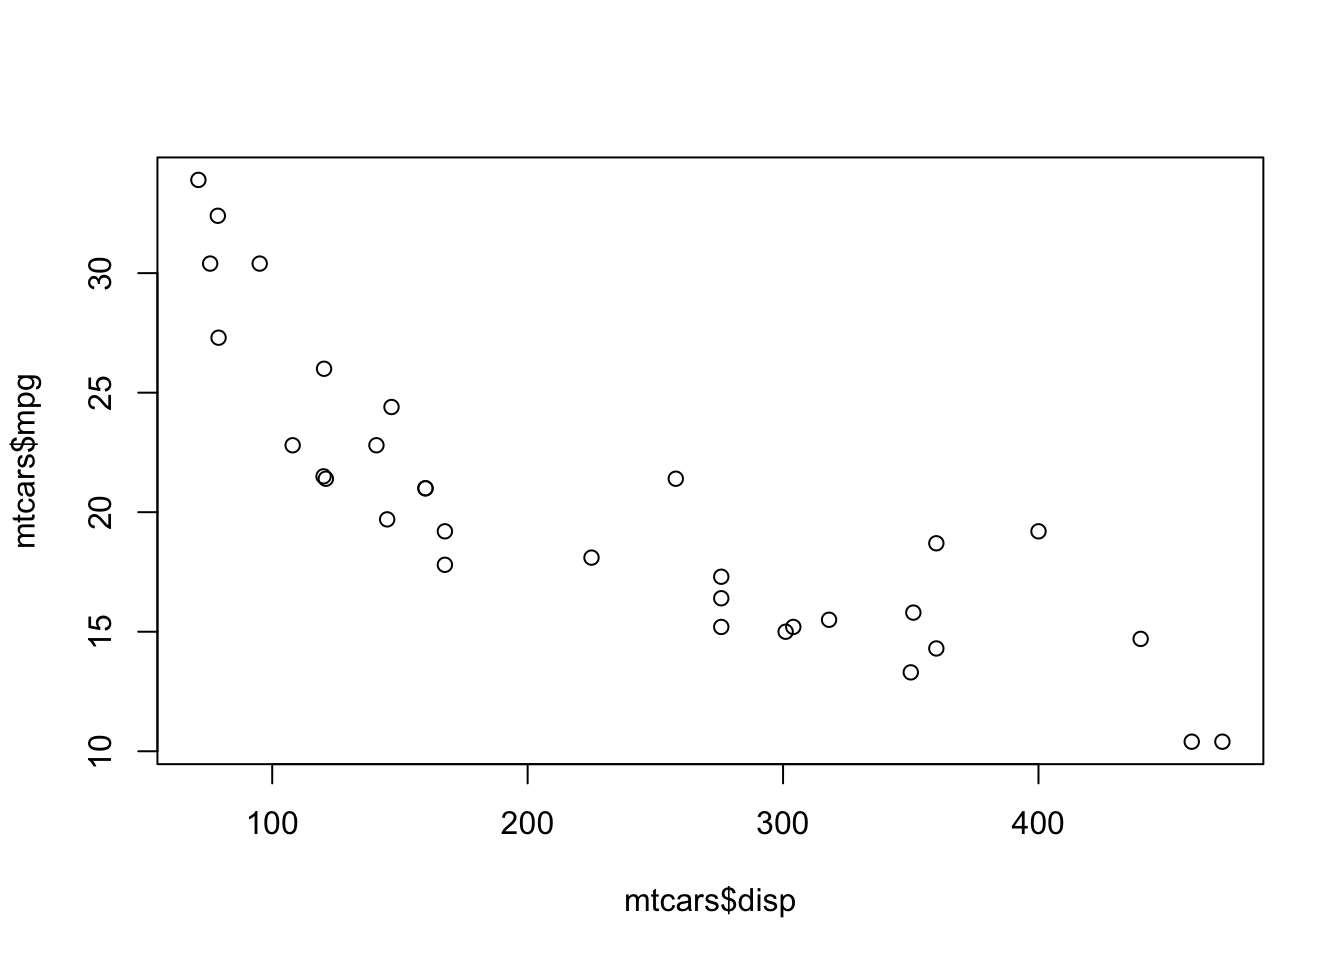
\includegraphics{bookdown-demo_files/figure-latex/unnamed-chunk-3-1.pdf}

Dette er noter og opgaver til faget statistik, for erhvervsakademier og
grundlæggende statistik på videregående uddannelser.

\leavevmode\hypertarget{BlockName3}{}%
Hello world \(\alpha\)

Dette er noter og opgaver til faget statistik, for erhvervsakademier og
grundlæggende statistik på videregående uddannelser.

\begin{verbatim}
##                      mpg cyl  disp  hp drat    wt  qsec vs am gear carb
## Mazda RX4           21.0   6 160.0 110 3.90 2.620 16.46  0  1    4    4
## Mazda RX4 Wag       21.0   6 160.0 110 3.90 2.875 17.02  0  1    4    4
## Datsun 710          22.8   4 108.0  93 3.85 2.320 18.61  1  1    4    1
## Hornet 4 Drive      21.4   6 258.0 110 3.08 3.215 19.44  1  0    3    1
## Hornet Sportabout   18.7   8 360.0 175 3.15 3.440 17.02  0  0    3    2
## Valiant             18.1   6 225.0 105 2.76 3.460 20.22  1  0    3    1
## Duster 360          14.3   8 360.0 245 3.21 3.570 15.84  0  0    3    4
## Merc 240D           24.4   4 146.7  62 3.69 3.190 20.00  1  0    4    2
## Merc 230            22.8   4 140.8  95 3.92 3.150 22.90  1  0    4    2
## Merc 280            19.2   6 167.6 123 3.92 3.440 18.30  1  0    4    4
## Merc 280C           17.8   6 167.6 123 3.92 3.440 18.90  1  0    4    4
## Merc 450SE          16.4   8 275.8 180 3.07 4.070 17.40  0  0    3    3
## Merc 450SL          17.3   8 275.8 180 3.07 3.730 17.60  0  0    3    3
## Merc 450SLC         15.2   8 275.8 180 3.07 3.780 18.00  0  0    3    3
## Cadillac Fleetwood  10.4   8 472.0 205 2.93 5.250 17.98  0  0    3    4
## Lincoln Continental 10.4   8 460.0 215 3.00 5.424 17.82  0  0    3    4
## Chrysler Imperial   14.7   8 440.0 230 3.23 5.345 17.42  0  0    3    4
## Fiat 128            32.4   4  78.7  66 4.08 2.200 19.47  1  1    4    1
## Honda Civic         30.4   4  75.7  52 4.93 1.615 18.52  1  1    4    2
## Toyota Corolla      33.9   4  71.1  65 4.22 1.835 19.90  1  1    4    1
## Toyota Corona       21.5   4 120.1  97 3.70 2.465 20.01  1  0    3    1
## Dodge Challenger    15.5   8 318.0 150 2.76 3.520 16.87  0  0    3    2
## AMC Javelin         15.2   8 304.0 150 3.15 3.435 17.30  0  0    3    2
## Camaro Z28          13.3   8 350.0 245 3.73 3.840 15.41  0  0    3    4
## Pontiac Firebird    19.2   8 400.0 175 3.08 3.845 17.05  0  0    3    2
## Fiat X1-9           27.3   4  79.0  66 4.08 1.935 18.90  1  1    4    1
## Porsche 914-2       26.0   4 120.3  91 4.43 2.140 16.70  0  1    5    2
## Lotus Europa        30.4   4  95.1 113 3.77 1.513 16.90  1  1    5    2
## Ford Pantera L      15.8   8 351.0 264 4.22 3.170 14.50  0  1    5    4
## Ferrari Dino        19.7   6 145.0 175 3.62 2.770 15.50  0  1    5    6
## Maserati Bora       15.0   8 301.0 335 3.54 3.570 14.60  0  1    5    8
## Volvo 142E          21.4   4 121.0 109 4.11 2.780 18.60  1  1    4    2
\end{verbatim}

\protect\hyperlink{anchors-in-markdown}{\# create an anchor}

\protect\hyperlink{anchors-in-markdown2}{create an anchor2}

 Orley Ashenfelter en Princeton økonom udviklede i 1980'erne en
statistik model til forudsigelse af vinpriser baseret på nedbør,
solskinstimer og andre klimadata. Hele den etablerede vinverden var i
oprør, ved en præsentation i Christie's vinafdeling, blev han buhet ud.
Robert Parker den verdenskendte vinkender udtalte ``Det svarer til en
filmanmelder der ikke ser filmen, men udelukkende baserer sin anmeldelse
på instruktøren og skuespilleren''. Orley udtalte, lang tid før det var
muligt for vinseksperterne, at 1989 Bordeux ville blive århundredets
vin, uanset den kun havde ligget 3 måneder på fade. Flere analyser har
siden vist Orleys model er langt mere præcis eksperterne. Meget få
vinkendere har anerkendt kvaliteten af Orleys model, men deres forecasts
ligger nu langt tættere på modellens forudsigelser.

Bogen er opbygget med en del praktiske eksempler.

Der er i nogle afsnit knapper med spørgsmål og svar, man kan klikke på
disse og se om man kan nå frem til de rigtige løsninger.

Bogen er bygget op så kapitlerne beskriver fanerne i Freestat
programmet. Man kan se og hente excelfiler direkte ved at klikke på
links.

\hypertarget{freestat-44}{%
\subsubsection{Freestat 44}\label{freestat-44}}

Man kan få beregnet deskriptorerne i et utal af programmer heriblandt
Freestat, der kan hentes herunder. Freestat kan gennemføre de mest
almindelige statistiske analyser, der er flere forskellige versioner.

\begin{quote}
block quote
\end{quote}

\href{https://www.dropbox.com/s/a2jztexbxfzcli0/FREESTAT.xlsx?dl=1}{Hent
Freestat til finansøkonomer her}

\href{https://www.dropbox.com/s/th8q95lf864npie/FREESTATfin.xlsx?dl=1}{Hent
Freestat fuld version her}

Take me to \protect\hyperlink{pookie}{pookie} And the destination
anchor:

Der findes opgaver quizzes og yderligere resourcer på
\href{http://www.edutest.dk}{www.edutest.dk}

Min gode ven Benjamin Tejlbjerg har lavet en super hjemmeside med
gymnasie matematik og statistik
\href{http://www.mathhx.dk/?q=node/117}{http://www.mathhx.dk}. Siden er
gratis og god til at genopfriske basisbegreber indenfor statistik, vi
kommer ikke i dybden med disse begreber her.

For at få et overblik over hypoteserne for de forskellige tests kan man
hente et hypotese mindmap, der er mindmaps til flere forskellige
uddannelser under materialer. Her er hypoteseoversigten for
finansøkonomer:
\href{https://drive.google.com/uc?export=download\&id=0B1E7VnhxsDMlQ1Zhdjh5WTJ4bnM}{CPH
Finansøkonom statistik mindmap}

Dette er 1. udgave af bogen, der tages forbehold for tryk og tastefejl,
men alle fejl eller uklarheder i måtte finde rettes med fluks. Forslag
til forbedringer modtages med kyshånd.

Der er en samlet oversigt over materialerne, der bruges i denne bog,
disse ligger i som linket materialer i menuen for oven.

\hypertarget{hvad-bruger-man-statistik-til.44}{%
\subsection{Hvad bruger man statistik
til.44}\label{hvad-bruger-man-statistik-til.44}}

I alle brancher i den finansielle sektor spiller statistik en rolle.

\begin{Shaded}
\begin{Highlighting}[]
\KeywordTok{library}\NormalTok{(DT)}
\KeywordTok{datatable}\NormalTok{(mtcars)}
\end{Highlighting}
\end{Shaded}

\includegraphics{bookdown-demo_files/figure-latex/unnamed-chunk-5-1.pdf}

\includegraphics{bookdown-demo_files/figure-latex/unnamed-chunk-6-1.pdf}

Bankerne sammensætter investeringsporteføljer, der minimerer risikoen
(variansen), ved aktiver der har lav eller negativ samvariation
(kovarians). Cykliske aktier som FL Smidth har fx. lav samvariation med
en ikke cyklisk aktie som Novo.

Forsikringsselskaberne beregner præmier for forsikringstageren, baseret
på statistike sandsynligheder for at en hændelse indtræffer. Modellerne
kan være meget specifikke, en indboforsikring kan fx. være baseret på
ikke bare postnummer, boligform, men også etage, uddannelsesniveau etc.

Finansielle virksomheder underlagt finanstilsynet, bruger modeller til
beregning af risiko baseret på statistisk analyse.

Mægleren beregner udbudspriser, udfra en multipel lineær
regressionsmodel, der indeholder variable som størrelse, energimærke,
tagtype etc.

\begin{center}\rule{0.5\linewidth}{\linethickness}\end{center}

\textbf{\emph{Noterne er kun til personligt brug. Alle rettigheder
forbeholdes. Fotografisk eller anden gengivelse af eller kopiering eller
anden udnyttelse, er uden forfatterens skriftlige samtykke forbudt
ifølge dansk lov om ophavsret.}}

\hypertarget{datast-og-data44}{%
\chapter{Datasæt og data44}\label{datast-og-data44}}

\hypertarget{uni--bi--og-multivariate-datast44}{%
\subsection{Uni- bi- og multivariate
datasæt44}\label{uni--bi--og-multivariate-datast44}}

Datasæt er sæt af en eller flere variable:

\begin{itemize}
\tightlist
\item
  Univariate datasæt fx tider ved marathonløb\\
\item
  Bivariate datasæt fx tider ved marathonløb og køn
\item
  Multivariate datasæt fx tider ved marathonløb, køn, alder, medlem af
  sports klub.
\end{itemize}

\hypertarget{kvalitative-variable33}{%
\subsection{Kvalitative variable33}\label{kvalitative-variable33}}

Kvalitative variable er data vi ikke kan måle eller tælle. De antager
værdier i form af navne eller labels:

\begin{itemize}
\tightlist
\item
  Kæledyr: kat, hund, marsvin
\item
  Køn: mand, kvinde
\item
  Favorit app: Angry Birds, Messenger, Audible, Tinder
\end{itemize}

\hypertarget{kvantitative-variable33}{%
\subsection{Kvantitative variable33}\label{kvantitative-variable33}}

Kvantitative variable er målbare numeriske variable, vi deler disse op i
\emph{kontinuerte} og \emph{diskrete} variable

\hypertarget{diskrete-variable33}{%
\subsubsection{Diskrete variable33}\label{diskrete-variable33}}

Diskrete variable er fx.

\begin{itemize}
\tightlist
\item
  Antal biler der passerer en bro observeret over flere dage.
\item
  Dagsproduktionen af chokoladefrøer på Toms. 
\item
  Antal personer der har iphones
\item
  Antallet af indbyggere i en by
\end{itemize}

\hypertarget{kontinuerte-variable33}{%
\subsubsection{Kontinuerte variable33}\label{kontinuerte-variable33}}

Kontinuerte variable er fx.

\begin{itemize}
\tightlist
\item
  Antal ml. indhold i shampoo flasker
\item
  Aktiekurser for Intel
\item
  Vægten på værnepligtige
\item
  Højden på studerende
\end{itemize}

\begin{Shaded}
\begin{Highlighting}[]
\KeywordTok{library}\NormalTok{(shiny)}

\KeywordTok{textInput}\NormalTok{(}\StringTok{"name"}\NormalTok{, }\StringTok{"What is your name?"}\NormalTok{)}
\end{Highlighting}
\end{Shaded}

What is your name?

\begin{Shaded}
\begin{Highlighting}[]
\KeywordTok{numericInput}\NormalTok{(}\StringTok{"age"}\NormalTok{, }\StringTok{"How old are you?"}\NormalTok{, }\OtherTok{NA}\NormalTok{, }\DataTypeTok{min =} \DecValTok{0}\NormalTok{, }\DataTypeTok{max =} \DecValTok{150}\NormalTok{)}
\end{Highlighting}
\end{Shaded}

How old are you?

\hypertarget{skalatyper33}{%
\subsection{Skalatyper33}\label{skalatyper33}}

Vi kan ydermere inddele variable efter skalatype hvor lavere betyder
mindst restriktiv.

\begin{enumerate}
\def\labelenumi{\arabic{enumi}.}
\tightlist
\item
  Nominalskala, bruges til at måle kvalitative data (er der kun 2 mulige
  udfald kaldes variablen specielt binær eller dikotom), fx.

  \begin{itemize}
  \tightlist
  \item
    Køn Mand Kvinde\\
  \item
    Styresystem: IOS Android Windows Symbian Andet
  \item
    Race: Europæisk, Afrikansk, Asiatisk Andet
  \end{itemize}
\item
  Ordinalskala inddeler data efter en rangordning

  \begin{itemize}
  \tightlist
  \item
    Karakterer på 7 trins skalaen -3 00 02\ldots{}
  \item
    Moodys credit ratings Aaa Aa A Baa Ba B Caa Ca C
  \item
    Tilfredshed meget utilfreds, noget utilfreds, nogenlunde tilfreds,
    meget tilfreds
  \end{itemize}
\item
  Intervalskala man kan sammenligne afstande og forskelle, men der er
  intet meningsfuldt nulpunkt. Nul for en intervalskala variabel betyder
  således ikke fravær af den målte størrelse. Nul grader celsius betyder
  altså ikke fravær af temperatur (det absolutte nulpunkt 0 Kelvin, hvor
  alle molekyler og atomer er i grundtilstanden). En IQ på 0 betyder
  ikke fravær af intelligens.

  \begin{itemize}
  \tightlist
  \item
    Temperatur målt i Celsius 
  \item
    Temperatur målt i Fahrenheit
  \item
    PH
  \item
    IQ
  \end{itemize}
\item
  Ratioskala

  \begin{itemize}
  \tightlist
  \item
    Beløb i lommen
  \item
    Højde på studerende
  \item
    Hastighed af biler ved vejkryds
  \item
    Indhold i Coca Cola flasker 
  \end{itemize}
\end{enumerate}

``Statistics are used much like a drunk uses a lamppost: for support,
not illumination.''\\
- Vin Scully

Interval- og ratioskalaer omtales som numeriske eller kontinuerte
skalaer, disse er knyttet til kvantitative variable.\\
Nominal- og ordinalskalaer omtales ofte som kategorisk eller faktor,
disse er knyttet til kvalitative variable.

En stikprøve af skalatype ratio kan fx. reduceres til ordinal, eller
nominal. Temperatur målt i celsius kan fx. omskrives til en ordinal
variabel: koldt normalt varmt, eller en nominal variabel: ekstrem
temperatur eller normal temperatur.

Kategoriske skalaer kan yderligere reduceres til en dikotom skala, ved
at sammenlægge kategorierne, til man kun har 2 kategorier.

Det er vanskeligere at ændre en nominal- ordinal- eller ratioskala til
en intervalskala. At ændre variablen nominalskala variablen køn til
ordinal giver fx. ikke mening.

\hypertarget{deskriptorer-freestat-33}{%
\paragraph{Deskriptorer Freestat 33}\label{deskriptorer-freestat-33}}

\hypertarget{freestat-33}{%
\subsubsection{Freestat 33}\label{freestat-33}}

Man kan få beregnet deskriptorerne i et utal af programmer heriblandt
Freestat, der kan hentes herunder. Freestat kan gennemføre de mest
almindelige statistiske analyser, der er flere forskellige versioner.

\href{https://www.dropbox.com/s/a2jztexbxfzcli0/FREESTAT.xlsx?dl=1}{Hent
Freestat til finansøkonomer her}

\href{https://www.dropbox.com/s/th8q95lf864npie/FREESTATfin.xlsx?dl=1}{Hent
Freestat fuld version her}

Der findes opgaver quizzes og yderligere resourcer på
\href{http://www.edutest.dk}{www.edutest.dk}

Min gode ven Benjamin Tejlbjerg har lavet en super hjemmeside med
gymnasie matematik og statistik
\href{http://www.mathhx.dk/?q=node/117}{http://www.mathhx.dk}. Siden er
gratis og god til at genopfriske basisbegreber indenfor statistik, vi
kommer ikke i dybden med disse begreber her.

For at få et overblik over hypoteserne for de forskellige tests kan man
hente et hypotese mindmap, der er mindmaps til flere forskellige
uddannelser under materialer. Her er hypoteseoversigten for
finansøkonomer:
\href{https://drive.google.com/uc?export=download\&id=0B1E7VnhxsDMlQ1Zhdjh5WTJ4bnM}{CPH
Finansøkonom statistik mindmap}

Dette er 1. udgave af bogen, der tages forbehold for tryk og tastefejl,
men alle fejl eller uklarheder i måtte finde rettes med fluks. Forslag
til forbedringer modtages med kyshånd.

Der er en samlet oversigt over materialerne, der bruges i denne bog,
disse ligger i som linket materialer i menuen for oven.

\hypertarget{hvad-bruger-man-statistik-til.33}{%
\subsection{Hvad bruger man statistik
til.33}\label{hvad-bruger-man-statistik-til.33}}

I alle brancher i den finansielle sektor spiller statistik en rolle.

Bankerne sammensætter investeringsporteføljer, der minimerer risikoen
(variansen), ved aktiver der har lav eller negativ samvariation
(kovarians). Cykliske aktier som FL Smidth har fx. lav samvariation med
en ikke cyklisk aktie som Novo.

Forsikringsselskaberne beregner præmier for forsikringstageren, baseret
på statistike sandsynligheder for at en hændelse indtræffer. Modellerne
kan være meget specifikke, en indboforsikring kan fx. være baseret på
ikke bare postnummer, boligform, men også etage, uddannelsesniveau etc.

Finansielle virksomheder underlagt finanstilsynet, bruger modeller til
beregning af risiko baseret på statistisk analyse.

Mægleren beregner udbudspriser, udfra en multipel lineær
regressionsmodel, der indeholder variable som størrelse, energimærke,
tagtype etc.

\begin{center}\rule{0.5\linewidth}{\linethickness}\end{center}

\textbf{\emph{Noterne er kun til personligt brug. Alle rettigheder
forbeholdes. Fotografisk eller anden gengivelse af eller kopiering eller
anden udnyttelse, er uden forfatterens skriftlige samtykke forbudt
ifølge dansk lov om ophavsret.}}

\hypertarget{datast-og-data22}{%
\chapter{Datasæt og data22}\label{datast-og-data22}}

\hypertarget{uni--bi--og-multivariate-datast22}{%
\subsection{Uni- bi- og multivariate
datasæt22}\label{uni--bi--og-multivariate-datast22}}

Datasæt er sæt af en eller flere variable:

\begin{itemize}
\tightlist
\item
  Univariate datasæt fx tider ved marathonløb\\
\item
  Bivariate datasæt fx tider ved marathonløb og køn
\item
  Multivariate datasæt fx tider ved marathonløb, køn, alder, medlem af
  sports klub
\end{itemize}

\hypertarget{kvalitative-variable-22}{%
\subsection{Kvalitative variable 22}\label{kvalitative-variable-22}}

Kvalitative variable er data vi ikke kan måle eller tælle. De antager
værdier i form af navne eller labels:

\begin{itemize}
\tightlist
\item
  Kæledyr: kat, hund, marsvin
\item
  Køn: mand, kvinde
\item
  Favorit app: Angry Birds, Messenger, Audible, Tinder
\end{itemize}

\hypertarget{kvantitative-variable55}{%
\subsection{Kvantitative variable55}\label{kvantitative-variable55}}

Kvantitative variable er målbare numeriske variable, vi deler disse op i
\emph{kontinuerte} og \emph{diskrete} variable

\hypertarget{diskrete-variable55}{%
\subsubsection{Diskrete variable55}\label{diskrete-variable55}}

Diskrete variable er fx.

\begin{itemize}
\tightlist
\item
  Antal biler der passerer en bro observeret over flere dage.
\item
  Dagsproduktionen af chokoladefrøer på Toms. 
\item
  Antal personer der har iphones
\item
  Antallet af indbyggere i en by
\end{itemize}

\hypertarget{kontinuerte-variable55}{%
\subsubsection{Kontinuerte variable55}\label{kontinuerte-variable55}}

Kontinuerte variable er fx.

\begin{itemize}
\tightlist
\item
  Antal ml. indhold i shampoo flasker
\item
  Aktiekurser for Intel
\item
  Vægten på værnepligtige
\item
  Højden på studerende
\end{itemize}

\hypertarget{skalatyper55}{%
\subsection{Skalatyper55}\label{skalatyper55}}

Vi kan ydermere inddele variable efter skalatype hvor lavere betyder
mindst restriktiv.

\begin{enumerate}
\def\labelenumi{\arabic{enumi}.}
\tightlist
\item
  Nominalskala, bruges til at måle kvalitative data (er der kun 2 mulige
  udfald kaldes variablen specielt binær eller dikotom), fx.

  \begin{itemize}
  \tightlist
  \item
    Køn Mand Kvinde\\
  \item
    Styresystem: IOS Android Windows Symbian Andet
  \item
    Race: Europæisk, Afrikansk, Asiatisk Andet
  \end{itemize}
\item
  Ordinalskala inddeler data efter en rangordning

  \begin{itemize}
  \tightlist
  \item
    Karakterer på 7 trins skalaen -3 00 02\ldots{}
  \item
    Moodys credit ratings Aaa Aa A Baa Ba B Caa Ca C
  \item
    Tilfredshed meget utilfreds, noget utilfreds, nogenlunde tilfreds,
    meget tilfreds
  \end{itemize}
\item
  Intervalskala man kan sammenligne afstande og forskelle, men der er
  intet meningsfuldt nulpunkt. Nul for en intervalskala variabel betyder
  således ikke fravær af den målte størrelse. Nul grader celsius betyder
  altså ikke fravær af temperatur (det absolutte nulpunkt 0 Kelvin, hvor
  alle molekyler og atomer er i grundtilstanden). En IQ på 0 betyder
  ikke fravær af intelligens.

  \begin{itemize}
  \tightlist
  \item
    Temperatur målt i Celsius 
  \item
    Temperatur målt i Fahrenheit
  \item
    PH
  \item
    IQ
  \end{itemize}
\item
  Ratioskala

  \begin{itemize}
  \tightlist
  \item
    Beløb i lommen
  \item
    Højde på studerende
  \item
    Hastighed af biler ved vejkryds
  \item
    Indhold i Coca Cola flasker 
  \end{itemize}
\end{enumerate}

``Statistics are used much like a drunk uses a lamppost: for support,
not illumination.''\\
- Vin Scully

Interval- og ratioskalaer omtales som numeriske eller kontinuerte
skalaer, disse er knyttet til kvantitative variable.\\
Nominal- og ordinalskalaer omtales ofte som kategorisk eller faktor,
disse er knyttet til kvalitative variable.

En stikprøve af skalatype ratio kan fx. reduceres til ordinal, eller
nominal. Temperatur målt i celsius kan fx. omskrives til en ordinal
variabel: koldt normalt varmt, eller en nominal variabel: ekstrem
temperatur eller normal temperatur.

Kategoriske skalaer kan yderligere reduceres til en dikotom skala, ved
at sammenlægge kategorierne, til man kun har 2 kategorier.

Det er vanskeligere at ændre en nominal- ordinal- eller ratioskala til
en intervalskala. At ændre variablen nominalskala variablen køn til
ordinal giver fx. ikke mening.

\hypertarget{deskriptorer-freestat-55}{%
\paragraph{Deskriptorer Freestat 55}\label{deskriptorer-freestat-55}}

Vis indhold ææø

\leavevmode\hypertarget{BlockName2}{}%
Hello world \(\alpha\)

Her skriver vi noget bla bla bla

\begin{center}\rule{0.5\linewidth}{\linethickness}\end{center}

\begin{verbatim}
##      speed           dist       
##  Min.   : 4.0   Min.   :  2.00  
##  1st Qu.:12.0   1st Qu.: 26.00  
##  Median :15.0   Median : 36.00  
##  Mean   :15.4   Mean   : 42.98  
##  3rd Qu.:19.0   3rd Qu.: 56.00  
##  Max.   :25.0   Max.   :120.00
\end{verbatim}

\hypertarget{indledning-start}{%
\chapter{Indledning Start}\label{indledning-start}}

Open me!

Pellentesque habitant morbi tristique senectus et netus et malesuada
fames ac turpis egestas. Vestibulum tortor quam, feugiat vitae,
ultricies eget, tempor sit amet, ante. Donec eu libero sit amet quam
egestas semper. Aenean ultricies mi vitae est. Mauris placerat eleifend
leo. Quisque sit amet est et sapien ullamcorper pharetra. Vestibulum
erat wisi, condimentum sed, commodo vitae, ornare sit amet, wisi. Aenean
fermentum, elit eget tincidunt condimentum, eros ipsum rutrum orci,
sagittis tempus lacus enim ac dui. Donec non enim in turpis pulvinar
facilisis. Ut felis.

Spørgsmål 1 whatever

Svar 1 whatever

Spørgsmål whatever

Spørgsmål whatever

\hypertarget{does-ruby-work-with-knitr}{%
\section{\texorpdfstring{Does Ruby work with
\textbf{knitr}?}{Does Ruby work with knitr?}}\label{does-ruby-work-with-knitr}}

\begin{Shaded}
\begin{Highlighting}[]
\NormalTok{x = }\StringTok{'hello, ruby world!'}
\NormalTok{p x.split(}\CharTok{' '}\NormalTok{)}
\end{Highlighting}
\end{Shaded}

\begin{verbatim}
## ["hello,", "ruby", "world!"]
\end{verbatim}

\hypertarget{js}{%
\section{js}\label{js}}

\hypertarget{bash}{%
\section{Bash}\label{bash}}

\begin{Shaded}
\begin{Highlighting}[]
\BuiltInTok{echo} \StringTok{"Hello Bash!"}
\FunctionTok{ls}
\end{Highlighting}
\end{Shaded}

\begin{verbatim}
## Hello Bash!
## 01-intro.Rmd
## 02-literature.Rmd
## 03-method.Rmd
## 04-application.Rmd
## 05-summary.Rmd
## 06-references.Rmd
## 07-application-kopi.Rmd
## DESCRIPTION
## LICENSE
## README.md
## _book
## _bookdown.yml
## _bookdown_files
## _build.sh
## _deploy.sh
## _output.yml
## book.bib
## bookdown-demo.Rmd
## bookdown-demo.Rproj
## bookdown-demo_files
## img
## index.Rmd
## packages.bib
## preamble.tex
## style.css
## toc.css
\end{verbatim}

\begin{Shaded}
\begin{Highlighting}[]
\DataTypeTok{void}\NormalTok{ square(}\DataTypeTok{double}\NormalTok{ *x) \{}
\NormalTok{  *x = *x * *x;}
\NormalTok{\}}
\end{Highlighting}
\end{Shaded}

Test the \texttt{square()} function:

\begin{Shaded}
\begin{Highlighting}[]
\KeywordTok{.C}\NormalTok{(}\StringTok{'square'}\NormalTok{, }\DecValTok{9}\NormalTok{)}
\end{Highlighting}
\end{Shaded}

\begin{verbatim}
## [[1]]
## [1] 81
\end{verbatim}

\begin{Shaded}
\begin{Highlighting}[]
\KeywordTok{.C}\NormalTok{(}\StringTok{'square'}\NormalTok{, }\DecValTok{123}\NormalTok{)}
\end{Highlighting}
\end{Shaded}

\begin{verbatim}
## [[1]]
## [1] 15129
\end{verbatim}

\hypertarget{a-normal-r-code-chunk}{%
\section{A normal R code chunk}\label{a-normal-r-code-chunk}}

\begin{Shaded}
\begin{Highlighting}[]
\KeywordTok{library}\NormalTok{(reticulate)}
\NormalTok{x =}\StringTok{ }\DecValTok{42}
\KeywordTok{print}\NormalTok{(x)}
\end{Highlighting}
\end{Shaded}

\begin{verbatim}
## [1] 42
\end{verbatim}

\hypertarget{modify-an-r-variable}{%
\section{Modify an R variable}\label{modify-an-r-variable}}

In the following chunk, the value of \texttt{x} on the right hand side
is 42, which was defined in the previous chunk.

\begin{Shaded}
\begin{Highlighting}[]
\NormalTok{x =}\StringTok{ }\NormalTok{x }\OperatorTok{+}\StringTok{ }\DecValTok{12}
\KeywordTok{print}\NormalTok{(x)}
\end{Highlighting}
\end{Shaded}

\begin{verbatim}
## [1] 54
\end{verbatim}

\hypertarget{a-python-chunk}{%
\section{A Python chunk}\label{a-python-chunk}}

This works fine and as expected.

\begin{Shaded}
\begin{Highlighting}[]
\NormalTok{x }\OperatorTok{=} \DecValTok{42} \OperatorTok{*} \DecValTok{2}
\BuiltInTok{print}\NormalTok{(x) }
\end{Highlighting}
\end{Shaded}

\begin{verbatim}
## 84
\end{verbatim}

The value of \texttt{x} in the Python session is 84. It is not the same
\texttt{x} as the one in R.

\hypertarget{modify-a-python-variable}{%
\section{Modify a Python variable}\label{modify-a-python-variable}}

\begin{Shaded}
\begin{Highlighting}[]
\NormalTok{x }\OperatorTok{=}\NormalTok{ x }\OperatorTok{+} \DecValTok{18} 
\BuiltInTok{print}\NormalTok{(x)}
\end{Highlighting}
\end{Shaded}

\begin{verbatim}
## 102
\end{verbatim}

Retrieve the value of \texttt{x} from the Python session again:

\begin{Shaded}
\begin{Highlighting}[]
\NormalTok{py}\OperatorTok{$}\NormalTok{x}
\end{Highlighting}
\end{Shaded}

\begin{verbatim}
## [1] 102
\end{verbatim}

Assign to a variable in the Python session from R:

\begin{Shaded}
\begin{Highlighting}[]
\NormalTok{py}\OperatorTok{$}\NormalTok{y =}\StringTok{ }\DecValTok{1}\OperatorTok{:}\DecValTok{5}
\end{Highlighting}
\end{Shaded}

See the value of \texttt{y} in the Python session:

\begin{Shaded}
\begin{Highlighting}[]
\BuiltInTok{print}\NormalTok{(y)}
\end{Highlighting}
\end{Shaded}

\begin{verbatim}
## [1, 2, 3, 4, 5]
\end{verbatim}

\hypertarget{python-graphics}{%
\section{Python graphics}\label{python-graphics}}

You can draw plots using the \textbf{matplotlib} package in Python.

\begin{Shaded}
\begin{Highlighting}[]
\ImportTok{import}\NormalTok{ matplotlib.pyplot }\ImportTok{as}\NormalTok{ plt}
\NormalTok{plt.plot([}\DecValTok{0}\NormalTok{, }\DecValTok{2}\NormalTok{, }\DecValTok{1}\NormalTok{, }\DecValTok{4}\NormalTok{])}
\NormalTok{plt.show()}
\end{Highlighting}
\end{Shaded}

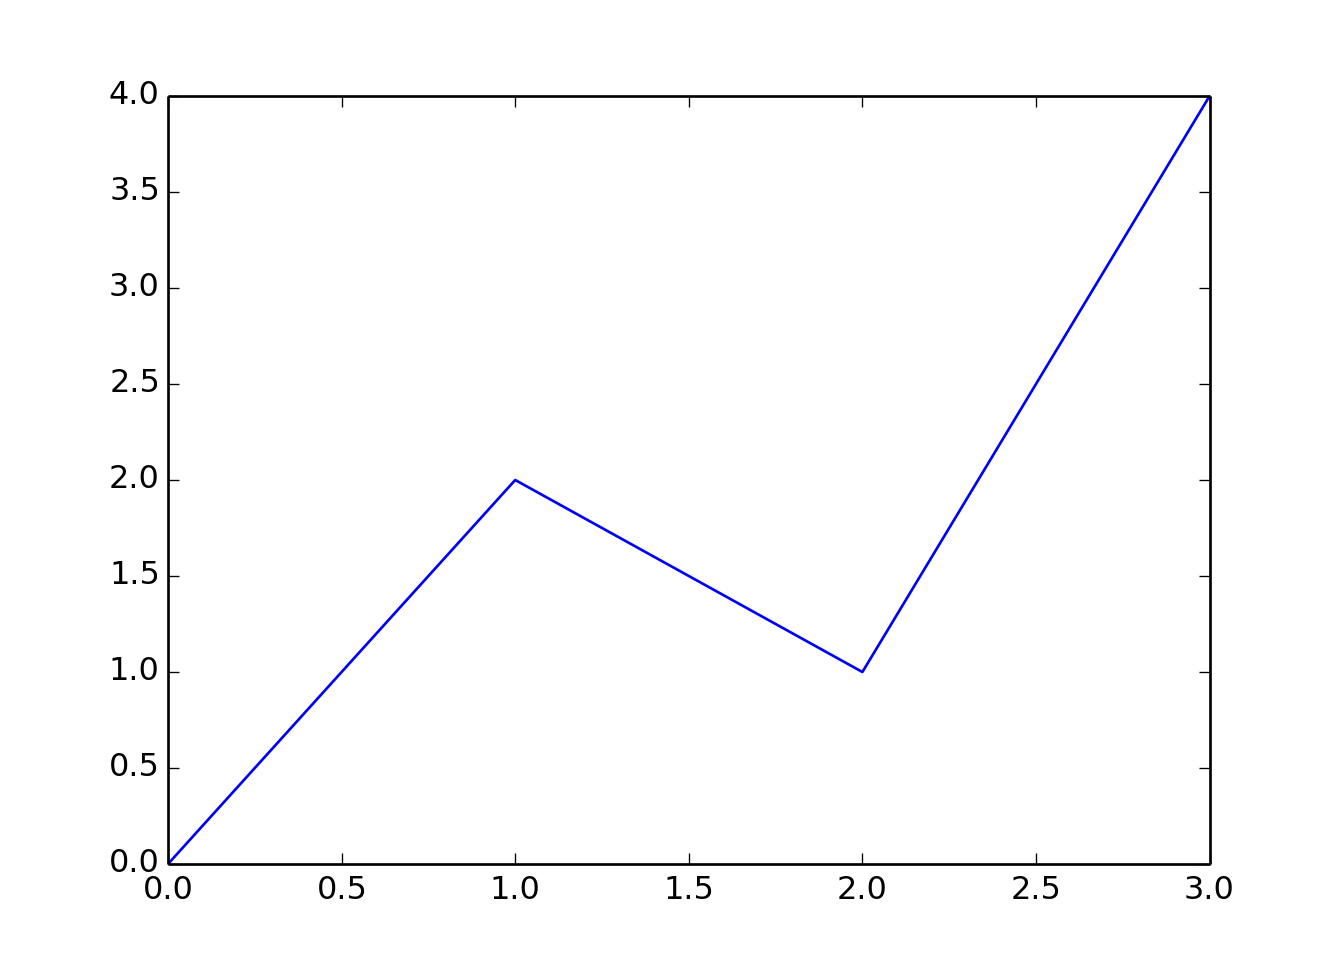
\includegraphics{bookdown-demo_files/figure-latex/unnamed-chunk-19-1.pdf}

Here is an inline note.\footnote{Inlines notes are easier to write,
  since you don't have to pick an identifier and move down to type the
  note.}

Here is an inline note.\footnote{2 Inlines notes are easier to write,
  since you don't have to pick an identifier and move down to type the
  note.}

The quick brown fox\footnote{Foxes are red} jumped over the lazy
dog\footnote{Dogs are usually not red}.

\begin{verbatim}
   Dette er en <span class="note" desc="lorem ut pretium malesuada, diam nunc interdum tellus, id venenatis tortor nulla eget lorem. Aenean pharetra imperdiet aliquam. Proin luctus nibh nec lobortis mattis. Sed egestas erat et urna egestas faucibus. Fusce porttitor dapibus tincidunt. Integer congue mattis nulla iaculis mollis.
\end{verbatim}

\begin{center}\rule{0.5\linewidth}{\linethickness}\end{center}

Dette er en \textless{}span class=``note'' desc="lorem ut pretium
malesuada, diam nunc interdum tellus, id venenatis tortor nulla eget
lorem. Aenean pharetra imperdiet aliquam. Proin luctus nibh nec lobortis
mattis. Sed egestas erat et urna egestas faucibus. Fusce porttitor
dapibus tincidunt. Integer congue mattis nulla iaculis mollis.

This is some text with a {marginal note}. Lorem ipsum dolor sit amet,
consectetur adipiscing elit. Nam consectetur, lorem ut pretium
malesuada, diam nunc interdum tellus, id venenatis tortor nulla eget
lorem. Aenean pharetra imperdiet aliquam. Proin luctus nibh nec lobortis
mattis. Sed egestas erat et urna egestas faucibus. Fusce porttitor
dapibus tincidunt. Integer congue mattis nulla iaculis mollis.

This is some text with a {marginal note}. Lorem ipsum dolor sit amet,
consectetur adipiscing elit. Nam consectetur, lorem ut pretium
malesuada, diam nunc interdum tellus, id venenatis tortor nulla eget
lorem. Aenean pharetra imperdiet aliquam. Proin luctus nibh nec lobortis
mattis. Sed egestas erat et urna egestas faucibus. Fusce porttitor
dapibus tincidunt. Integer congue mattis nulla iaculis mollis.

\hypertarget{opgaver}{%
\section{Opgaver}\label{opgaver}}

\hypertarget{sprgsmal-1}{%
\subsection{Spørgsmål 1}\label{sprgsmal-1}}

(tab content)

\hypertarget{svar-1}{%
\subsection{Svar 1}\label{svar-1}}

(tab content)

\hypertarget{sprgsmal-2}{%
\subsection{Spørgsmål 2}\label{sprgsmal-2}}

Spørgsmål 2

\hypertarget{sprgsmal-2-1}{%
\subsection{Spørgsmål 2}\label{sprgsmal-2-1}}

(Spørgsmål 2)

\hypertarget{quarterly-results}{%
\section{Quarterly Results}\label{quarterly-results}}

\hypertarget{sprgsmal-1-1}{%
\subsection{Spørgsmål 1}\label{sprgsmal-1-1}}

(tab content)

\hypertarget{svar-1-1}{%
\subsection{Svar 1}\label{svar-1-1}}

(tab content)

\hypertarget{sprgsmal-2-2}{%
\subsection{Spørgsmål 2}\label{sprgsmal-2-2}}

Spørgsmål 2

\hypertarget{sprgsmal-3}{%
\subsection{Spørgsmål 3}\label{sprgsmal-3}}

\[\frac{\beta}{\alpha+33}\] \# End tabs

\hypertarget{nyt-afsnit-efter-tabbed}{%
\section{Nyt afsnit efter tabbed}\label{nyt-afsnit-efter-tabbed}}

Plain text\\
End a line with two spaces to start a new paragraph.\\
\emph{italics} and \emph{italics}\\
\textbf{bold} and \textbf{bold}\\
superscript\textsuperscript{2}\\
\sout{strikethrough}\\
\href{www.rstudio.com}{link}\\
\# Header 1\\
\#\# Header 2\\
\#\#\# Header 3 \#\#\#\# Header 4 \#\#\#\#\# Header 5 \#\#\#\#\#\#
Header 6 endash: --\\
emdash: ---\\
ellipsis: \ldots{}\\
inline equation: \(A = \pi*r^{2}\)

\ldots{}

horizontal rule (or slide break): **\emph{ \textgreater{} block quote\\
} unordered list\\
* item 2\\
+ sub-item 1\\
+ sub-item 2

\begin{enumerate}
\def\labelenumi{\arabic{enumi}.}
\tightlist
\item
  ordered list\\
\item
  item 2\\
\end{enumerate}

\begin{itemize}
\tightlist
\item
  sub-item 1\\
\item
  sub-item 2
\end{itemize}

\begin{longtable}[]{@{}ll@{}}
\toprule
Table Header & Second Header\tabularnewline
\midrule
\endhead
Table Cell & Cell 2\tabularnewline
Cell 3 & Cell 4\tabularnewline
\bottomrule
\end{longtable}

\begin{center}\rule{0.5\linewidth}{\linethickness}\end{center}

\begin{center}\rule{0.5\linewidth}{\linethickness}\end{center}

You can label chapter and section titles using \texttt{\{\#label\}}
after them, e.g., we can reference Chapter \ref{intro}. If you do not
manually label them, there will be automatic labels anyway, e.g.,
Chapter \ref{methods}.

Figures and tables with captions will be placed in \texttt{figure} and
\texttt{table} environments, respectively.

\begin{Shaded}
\begin{Highlighting}[]
\KeywordTok{par}\NormalTok{(}\DataTypeTok{mar =} \KeywordTok{c}\NormalTok{(}\DecValTok{4}\NormalTok{, }\DecValTok{4}\NormalTok{, }\FloatTok{.1}\NormalTok{, }\FloatTok{.1}\NormalTok{))}
\KeywordTok{plot}\NormalTok{(pressure, }\DataTypeTok{type =} \StringTok{'b'}\NormalTok{, }\DataTypeTok{pch =} \DecValTok{19}\NormalTok{)}
\end{Highlighting}
\end{Shaded}

\begin{figure}

{\centering 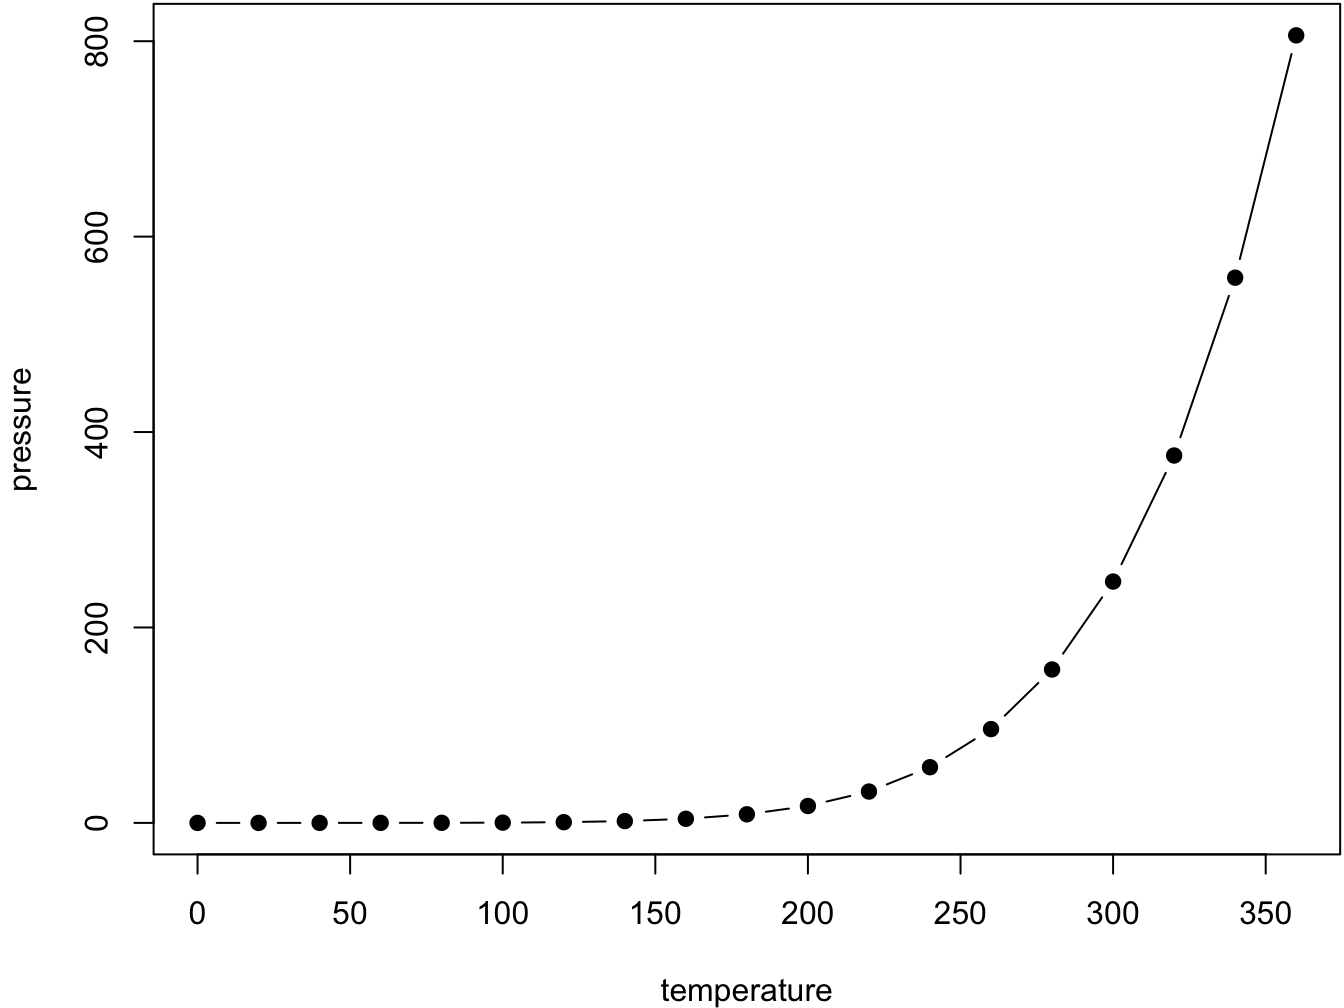
\includegraphics[width=0.8\linewidth]{bookdown-demo_files/figure-latex/nice-fig-1} 

}

\caption{Here is a nice figure!}\label{fig:nice-fig}
\end{figure}

Reference a figure by its code chunk label with the \texttt{fig:}
prefix, e.g., see Figure \ref{fig:nice-fig}. Similarly, you can
reference tables generated from \texttt{knitr::kable()}, e.g., see Table
\ref{tab:nice-tab}.

\begin{Shaded}
\begin{Highlighting}[]
\NormalTok{knitr}\OperatorTok{::}\KeywordTok{kable}\NormalTok{(}
  \KeywordTok{head}\NormalTok{(iris, }\DecValTok{20}\NormalTok{), }\DataTypeTok{caption =} \StringTok{'Here is a nice table!'}\NormalTok{,}
  \DataTypeTok{booktabs =} \OtherTok{TRUE}
\NormalTok{)}
\end{Highlighting}
\end{Shaded}

\begin{table}

\caption{\label{tab:nice-tab}Here is a nice table!}
\centering
\begin{tabular}[t]{rrrrl}
\toprule
Sepal.Length & Sepal.Width & Petal.Length & Petal.Width & Species\\
\midrule
5.1 & 3.5 & 1.4 & 0.2 & setosa\\
4.9 & 3.0 & 1.4 & 0.2 & setosa\\
4.7 & 3.2 & 1.3 & 0.2 & setosa\\
4.6 & 3.1 & 1.5 & 0.2 & setosa\\
5.0 & 3.6 & 1.4 & 0.2 & setosa\\
\addlinespace
5.4 & 3.9 & 1.7 & 0.4 & setosa\\
4.6 & 3.4 & 1.4 & 0.3 & setosa\\
5.0 & 3.4 & 1.5 & 0.2 & setosa\\
4.4 & 2.9 & 1.4 & 0.2 & setosa\\
4.9 & 3.1 & 1.5 & 0.1 & setosa\\
\addlinespace
5.4 & 3.7 & 1.5 & 0.2 & setosa\\
4.8 & 3.4 & 1.6 & 0.2 & setosa\\
4.8 & 3.0 & 1.4 & 0.1 & setosa\\
4.3 & 3.0 & 1.1 & 0.1 & setosa\\
5.8 & 4.0 & 1.2 & 0.2 & setosa\\
\addlinespace
5.7 & 4.4 & 1.5 & 0.4 & setosa\\
5.4 & 3.9 & 1.3 & 0.4 & setosa\\
5.1 & 3.5 & 1.4 & 0.3 & setosa\\
5.7 & 3.8 & 1.7 & 0.3 & setosa\\
5.1 & 3.8 & 1.5 & 0.3 & setosa\\
\bottomrule
\end{tabular}
\end{table}

You can write citations, too. For example, we are using the
\textbf{bookdown} package \citep{R-bookdown} in this sample book, which
was built on top of R Markdown and \textbf{knitr} \citep{xie2015}.

\hypertarget{literature}{%
\chapter{Literature}\label{literature}}

Here is a review of existing methods.

\hypertarget{methods}{%
\chapter{Methods}\label{methods}}

We describe our methods in this chapter.

\hypertarget{applications}{%
\chapter{Applications}\label{applications}}

Some \emph{significant} applications are demonstrated in this chapter.

\hypertarget{example-one}{%
\section{Example one}\label{example-one}}

\hypertarget{example-two}{%
\section{Example two}\label{example-two}}

\hypertarget{final-words}{%
\chapter{Final Words}\label{final-words}}

We have finished a nice book.

\hypertarget{applications-tilfjet}{%
\chapter{Applications tilføjet}\label{applications-tilfjet}}

Some \emph{significant} applications are demonstrated in this chapter.

\hypertarget{example-one-1}{%
\section{Example one}\label{example-one-1}}

Her er lidt tekst

\hypertarget{example-two-1}{%
\section{Example two}\label{example-two-1}}

Og her

\hypertarget{hvad-med-denne-linje}{%
\subsection{Hvad med denne linje?}\label{hvad-med-denne-linje}}

\bibliography{book.bib,packages.bib}


\end{document}
